Pearson correlations between the spiking activity of pairs of neurons, or simply \emph{neural correlations}, are among the most familiar descriptive statistics of neural population activity \cite{Averbeck:2006,Zohary:1994,Kohn:2005,Bair:2001,Renart:2010}.  For example, \emph{noise correlations}, \emph{i.e.}~the correlations of stimulus response variability between pairs of neurons, have been of particular interest.  Noise correlations can have profound theoretical implications for stimulus coding \cite{Zohary:1994,Abbott:1999,Averbeck:2006,Berens:2011,Ecker:2011}, and have been interpreted to indicate detailed and specific functional organization. Such interpretation is supported by a series of discoveries of nontrivial relationships between neural correlations and other aspects of circuit organization such as the physical distance separating the neurons \cite{Smith:2008,Denman:2013}, their synaptic connectivity and stimulus tuning similarity \cite{Kohn:2005,Ko:2011}, cortical layer specificity \cite{Hansen:2012,Smith:2013}, cell-type specificity (?), progressive changes in development and in learning \cite{Golshani:2009}, changes due to sensory stimulation and global brain states \cite{Goard:2009,Kohn:2009,Ecker:2010,Renart:2010}, and others.

However, neural correlations do not come with ready or unambiguous mechanistic interpretations.  Theoretical and simulation studies have shown that neural correlations may arise at various temporal scales from combinations of multiple underlying mechanisms.  These include direct synaptic interactions, common or correlated inputs, shared sensory noise, chains of multiple synaptic connections, oscillations, top-down modulation, and background network activity \cite{Perkel:1967b,Shadlen:1998,Salinas:2001,Ostojic:2009,Rosenbaum:2011}.

Early studies of neural correlations were based on measurements from isolated pairs of neurons and their impact on coding was extrapolated to entire populations \cite{Shadlen:1998,Zohary:1994}.  Multineuronal recordings allow estimation of covariance matrices of large populations of neurons.  Such estimates provide more information than the equivalent number of pairwise correlations assessed in isolation. Indeed, the correlation matrix is greater than the sum of its parts: it can be transformed into other representations that accentuate different aspects of the correlation structure and may suggest different mechanistic interpretations. For example, the eigenvalue decomposition of the covariance matrix expresses shared correlated activity components across the population; common fluctuations of population activity may be accurately represented by just a few principal components but will affect all correlation coefficients. In contrast, the off-diagonal elements of the inverse of the correlation matrix constitute scaled partial correlations between neuron pairs, which reflect their specific linear dependencies, after accounting for the activity of all the other recorded cells; a strong interaction between a pair of neurons may be expressed by a single partial correlation but its effects may propagate to multiple correlations and eigenvalues.   The inverse of the covariance matrix plays an important role in decoding schemes such as linear discriminant analysis, for example.  The mutliple  representations of the covariance matrix with their alternative interpretations add both complications and opportunities into the search for fundamental regularities in neural population activity. 

\begin{figure}[htp]
\begin{center}
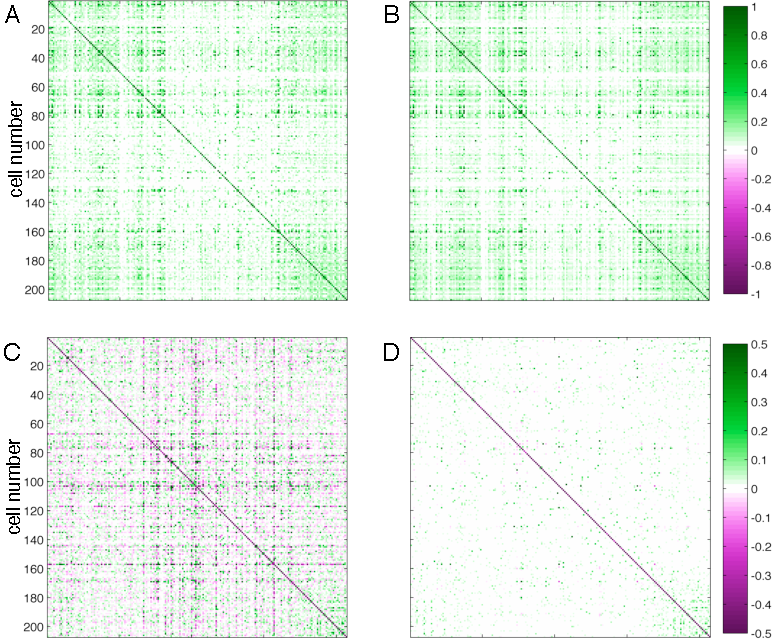
\includegraphics[width=0.5\textwidth]{figures/Figure0.pdf}
\end{center}
\caption{
{\bf An illustration of regularized estimaton of the covariance matrix.}  \TODO{generate a smaller and simple example}
{\bf A:} The sample covariance matrix of population calcium signals of 204 cells.
{\bf B:} The sample precison matrix (inverse of the sample covariance matrix in {\bf B}.
{\bf C:} A estimate of the covariance matrix produced by bounding the $L_1$ norm of the precision matrix. 
{\bf D:} The precision matrix of the estimate in {\bf C}.
}
\label{fig:00}
\end{figure}


With large numbers of recorded cells, the usual estimations of the covariance matrix from finite recordings become ill-conditioned. Numerical instabilities arise because, as the amount of recorded data increases only linearly, the number of free coefficients to be estimated in any parameterization of the covariance matrix increases quadratically. 
For example, the large eigenvalues of large sample covariance matrices are biased upward while small eigenvalues are biased downward \cite{Ledoit:2004}. Similarly, the coefficients of the inverse covariance matrix require larger sample sizes to be estimated accurately from high-dimensional data than low-dimensional data.

With this study, we pursue two related goals: 
\begin{enumerate}
	\item Devise more efficient estimators of neural covariance matrices in recordings from large populations of neurons.
	\item Aid interpretation of neural covariance matrices.
\end{enumerate}

To select the best covariance matrix estimate for a specific neural circuit, we evaluate the performance of four estimators using different regularization schemes, each motivated by  a different hypothesis for the origin of neural correlations. \emph{Regularization} is the deliberate biasing the solution toward a simplified, low-dimensional (`sparse') \emph{target estimate} \cite{Schafer:2005,Bickel:2006}.
Regularized estimators allow reaching a favorable tradeoff between bias and variance in order to minimize the total error.
Strikingly, some improvement can be produced even when the target estimate is chosen arbitrarily, which is sometimes described as ``Stein's phenomenon'' after its discoverer \cite{Stein:1956}.   However, when a sparse target estimate does happen to match the dominant features of the true covariance matrix, it will induce relatively little bias while retaining low variance.  For example, some covariance estimators have been motivated by a specific model of the underlying process such as single-factor models of the stock market, for example \cite{Ledoit:2003}. 
Since the true covariance structure is not known in practice, the performance of estimators is evaluated by how well their performance generalized to new data, outside the training sample by cross validation, for example. 


We compared the performance of several covariance estimators for spatially compact groups of 150--300 neurons in layers 2--4 in mouse primary visual cortex during visual stimulation.   The performance of the estimators was evaluated by computing the mean squared error between the optimized covariance estimate fitted to training data and the non-regularized covariance matrix from a separate test data set.  Low-rank covariance estimates performed significantly better than shrinkage estimators, but estimators with sparse partial correlations were more efficient still. Typically, between 3 and 16\% of neuronal pairs were connected by non-zero partial interactions.  Mixed sparse estimators with sparse partial correlations and low-rank components performed comparably. 

